\documentclass{article}           % Sets style/look of many things.
% \documentclass{report}          % part, chapters, front page etc.
\usepackage{exsheets}
\usepackage[utf8]{inputenc}       % Encoding of input files UTF-8
\usepackage[T1]{fontenc}
\usepackage[scaled]{beramono}     % Font
\usepackage{color}                % Color text
\usepackage{titlesec}             % Select alternative section titles
\usepackage{fancyvrb}
\usepackage{verbatim}             % Comment environment
\usepackage{listings}             % Format and render text/code etc.
\usepackage{minted}               % Much better syntax highlighting
\usepackage{float}                % Control of floating environment/figure
\usepackage{graphicx,  subfigure} % Better figures, graphics, units etc.
\usepackage{multicol}             % Multiple columns
\usepackage{amsmath}              % Math: Equation, split, align etc.
\usepackage{siunitx}              % SI units
\usepackage{mathtools}            % Different math tools to use with amsmath
\usepackage{amssymb}              % Math symbols
\usepackage[
    colorlinks,
    citecolor=black,              % I like links with standard black color
    filecolor=black,
    linkcolor=black,
    urlcolor=black
]{hyperref}                       % Links in TOC etc.
\usepackage[all]{hypcap}          % Better links to floating environment

\usepackage{tabto}
\newcommand\marginsymbol[1][0pt]{%
    \tabto*{0cm}\makebox[\dimexpr-1cm-#1\relax][r]{$\mathbb{P}$}\tabto*{\TabPrevPos}}

\renewcommand{\thesubsection}{\thesection.\alph{subsection}}

% Make margins smaller to fit more figures, tables etc on page: (optional)
\addtolength{\oddsidemargin}{-1.0in}
\addtolength{\evensidemargin}{-1.0in}
\addtolength{\textwidth}{2.0in}
\addtolength{\topmargin}{-0.8in}
\addtolength{\textheight}{1.6in}

\title{\vspace{-2cm}INF3490/INF4490 Exercise Solutions - Advanced Neural Networks}
\author{Eivind Samuelsen\footnote{See \href{https://github.com/olehermanse/INF3490-AI_Machine_Learning/blob/master/README.md}{\textbf{README}} for complete list of authors/contributors.}
}
\date{}

% Removing paragraph indents is sometimes useful:
% \setlength\parindent{0pt}
% ==============================================================================

% ================================= DOCUMENT ===================================
\begin{document}
    \renewcommand\marginsymbol[1][0pt]{%
  \tabto*{0cm}\makebox[-1cm][c]{$\mathbb{P}$}\tabto*{\TabPrevPos}}

\maketitle
\(\mathbb{P}\) marks the programming exercises, we strongly recommend using
the python programming language for these. Exercises may be added/changed
after publishing.


\section{Perceptron activation functions}
Last week we used the activation function
\begin{equation}
g(h) =
\begin{cases}
1 & h > 0 \\
0 & h \leq 0
\end{cases}
\end{equation}
Why is this not used with backpropagation?\\

\noindent\textit{Answer:}

\noindent
Backpropagation is entirely dependent on the output of the neurons \emph{not} being hard zeroes and ones, so that it can make gradual changes to them.
From a technical perspective, it is dependent on the activation function \(y_i = f(a_i)\) being differentiable, with a derivative \(f'(a_i)\) that can be written as a function of the neuron output \(y_i\) (you could perhaps write it as \(g'(y_i) = f'(f^{-1}(yi))\)), in order to estimate how much the weighted sum of inputs \(a_i\) has to change in order to achieve a change in \(y_i\) that is proportional to the derivative of the error \(y_i - t_i\).

\section{Hidden layers}
What is the minimum number of hidden neuron layers needed in order to approximate an arbitrary continuous function, and why?\\

\noindent\textit{Answer:}

\noindent
You need three layers (one output layer plus two hidden layers) in order to create any decision boundary.
Take the two-dimensional case: one layer gives you straight lines, and two layers gives you any shape that is in between any number of lines, so any convex shape - which includes all triangles.
By combining enough triangles (remember, we haven’t put any limits on how many neurons we have in each layer) we can approximate any shape.
Luckily, this holds for any number of dimensions, so three layers is enough no matter how many input nodes we have.

\section{Validation}
Why do we use a validation set?
Describe how the three different cross-validation methods presented in the lecture slides work, and what their advantages and disadvantages are.\\

\noindent\textit{Answer:}

\noindent
First off, there has been some confusion about exactly what cross-validation means.
The lecture slides and the book describes it as something involving three sets: a training set, a validation set and a test set, and is described as something you do in order to implement early stopping.
Contrary to this, the cross-validation that you were to do in the second mandatory exercise only involves a training set and a test set, and isn’t used for early stopping at all!

The first definition is actually just an extension to cross-validation that is used in order to do early stopping properly.
In both cases we split up our data and use parts of it for training data while the rest remains “unseen” by the training, and is used for validating the training.
To better avoid bias, this data then has to be split into separate sets for evaluating when to stop training (the “validation set” in the lectures) and for evaluating final performance (the “test set” in the lectures).

In general then, a validation set is used in order to evaluate the performance of
the trained classifier on unseen data.
In accordance with the terminology used in
the book, it would also be valid to answer that the validation set is used to test for
when it is right to stop early.

The three validation methods work as follows:

\begin{itemize}
    \item Simple cross-validation: the data is simply split into two (three) equally large parts, with one part used for training, (one part used for determining early stopping) and one part used for final evaluation.
    \item k-fold cross-validation: the data is separated into k folds. The training is then done k times, each time using a different fold as the test data (or with early stopping: one fold for validation during training and one fold for the final evaluation) and the rest as training data.
    \item Leave one out cross-validation: in turn, leave out each single data sample and train on the rest, testing on the single sample you left out, and calculate the success rate. (kind of an extreme case of k-fold cross-validation).
\end{itemize}

\section{Multi Layer Perceptron}
Implement the MLP shown below, and train it to correctly perform the XOR function.

\begin{figure}[H]
\begin{center}
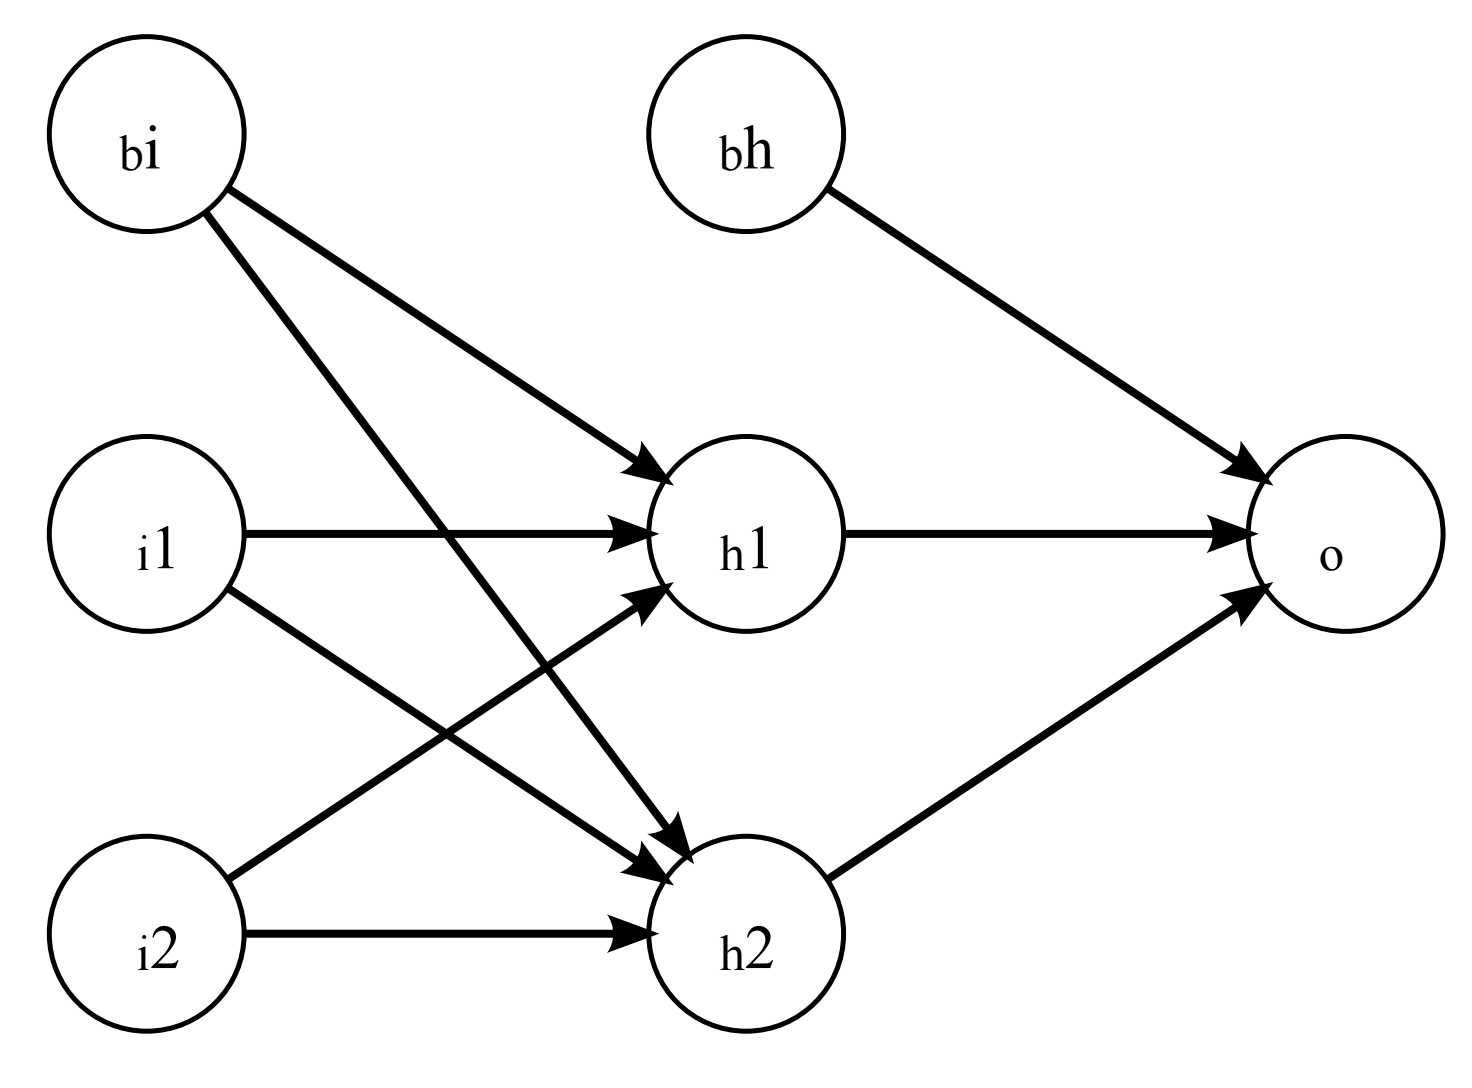
\includegraphics[width=0.4\textwidth]{mlp.png}
\caption{MLP with one hidden layer and two hidden nodes.}
\label{fig:mlp}
\end{center}
\end{figure}

\noindent\textit{Answer:}

\noindent
No solution given, as this is very similar to the mandatory assignment.

\section{Delta(error) function}
In the lecture slides the backpropagation deltas are first presented as
\[
\delta_k = (y_k - t_k)y_k(1-y_k)
\]
What does this tell us about the activation function in use?\\

\noindent\textit{Answer:}

\noindent
In general the backpropagation deltas are defined as \(\delta_k = (y_k - t_k)g'(y_k)\) where \(g'(y_k)\) is the derivative of the activation function as a function of the activation output as mentioned in the previous exercise.
In this case we have \(\delta_k = (y_k-t_k)y_k(1-y_k)\), so we must have \(g'(y_k) = y_k(1-y_k)\).
Then we would need to be either clever at math or hope that this is a common activation function so that we can find it in some text about neural networks.
In fact, this \(g'(y_k)\) corresponds to the single most common activation function:
\begin{equation}
    f(x) = \frac{1}{1+e^{-x}}
\end{equation}
The derivation goes like this:
\begin{align*}
    f'(x) &= \frac{e^{-x}}{(1+e^{-x})^2}\\
        a &= 1+e^{-x}\\
    f'(x) &= \frac{e^{-x}}{(a)^2}\\
    f'(x) &= \frac{1 + e^{-x} - 1}{(a)(a)}\\
    f'(x) &= \frac{a - 1}{(a)(a)}\\
    f'(x) &= \frac{a - 1}{(a)} \frac{1}{(a)}\\
    f'(x) &= (\frac{a}{a} - \frac{1}{a})\frac{1}{a}\\
    f'(x) &= (1 - \frac{1}{a})\frac{1}{a}\\
    f'(x) &= (1 - f(x))f(x)
\end{align*}

\section{Natural language MLP}
You are to design an MLP that would learn to hyphenate words correctly.
You would have a dictionary that shows correct hyphenation examples for lots of words.
Think about the following:
What should the input to the neural net be?
\begin{itemize}
    \item How should this input be encoded to work well with the classifier?
    \item How is should the output be encoded?
    \item How many layers do you need?
    \item How many neurons should there be in each layer?
\end{itemize}

\noindent\textit{Answer:}

\noindent
There are many ways of solving this, but the simplest way to arrange the input is to take pairs of letters as input, and assume that some external mechanism will feed us with candidate letter-pairs.

The next question is then how to encode the letter-pairs.
Neural networks takes their input as a fixed number of real-valued scalars.
So we need an encoding in that form.
But, there is no clear and easy way to put the relevant set of letters on a one-dimensional scale, or even a multidimensional scale.

What we can do is to use binary inputs: we encode each letter with one input for each possible value.
In the biological analogy of neural networks this would correspond to having a specialized neuron in our brain that detects a single letter.
E.g. in the English alphabet we would get 26 inputs per letter.
Then we want two letters as input, so we would get a total of 52 inputs to our neural net.

Finally, since we take pairs of letters as input, the output can simply be a true or false value that says whether this is a good place to hyphenate or not.
In that case, the output layer only needs to have one single neuron.

The number of hidden layers and their neuron count depends on how difficult we believe the problem to be.
We don’t expect there to be any easy patterns to which letter-pairs that are “hyphenatable”, so the classification problem is unlikely to be linearly separable, or maybe even separable by a convex shape, so it would probably be wise to have two hidden layers, so that the network can classify complex shapes in the input space.
The number of neurons in each layer would have to be up to experimentation, but a wise default value might be to reduce the number of neurons in each layer linearly, so if you have N inputs, you would have \(2N/3\) neurons in the first hidden layer and \(N/3\) neurons in the second.
Again, with the English alphabet, this would give \(104/3 \approx 35\) and \(52/3 \approx 17\) hidden nodes.

\section*{Contact and Github}
Corrections of grammar, language, notation or suggestions for improving this material are appreciated.
E-mail me at \href{mailto:olehelg@uio.no}{\textbf{olehelg@uio.no}} or use \href{https://github.com/olehermanse/INF3490-AI_Machine_Learning}{\textbf{GitHub}} to submit an issue or create a pull request.
The \href{https://github.com/olehermanse/INF3490-AI_Machine_Learning}{\textbf{GitHub repository}} contains all source code for assignments, exercises, solutions, examples etc.
As many people have been involved with writing and updating the course material, they are not all listed as authors here.
For a more complete list of authors and contributors see the \href{https://github.com/olehermanse/INF3490-AI_Machine_Learning/blob/master/README.md}{\textbf{README}}.

\end{document}
% ==============================================================================
